\label{section:foreign_relations_supervised_model}

\begin{figure}
  \center
  \vspace{-55pt}
  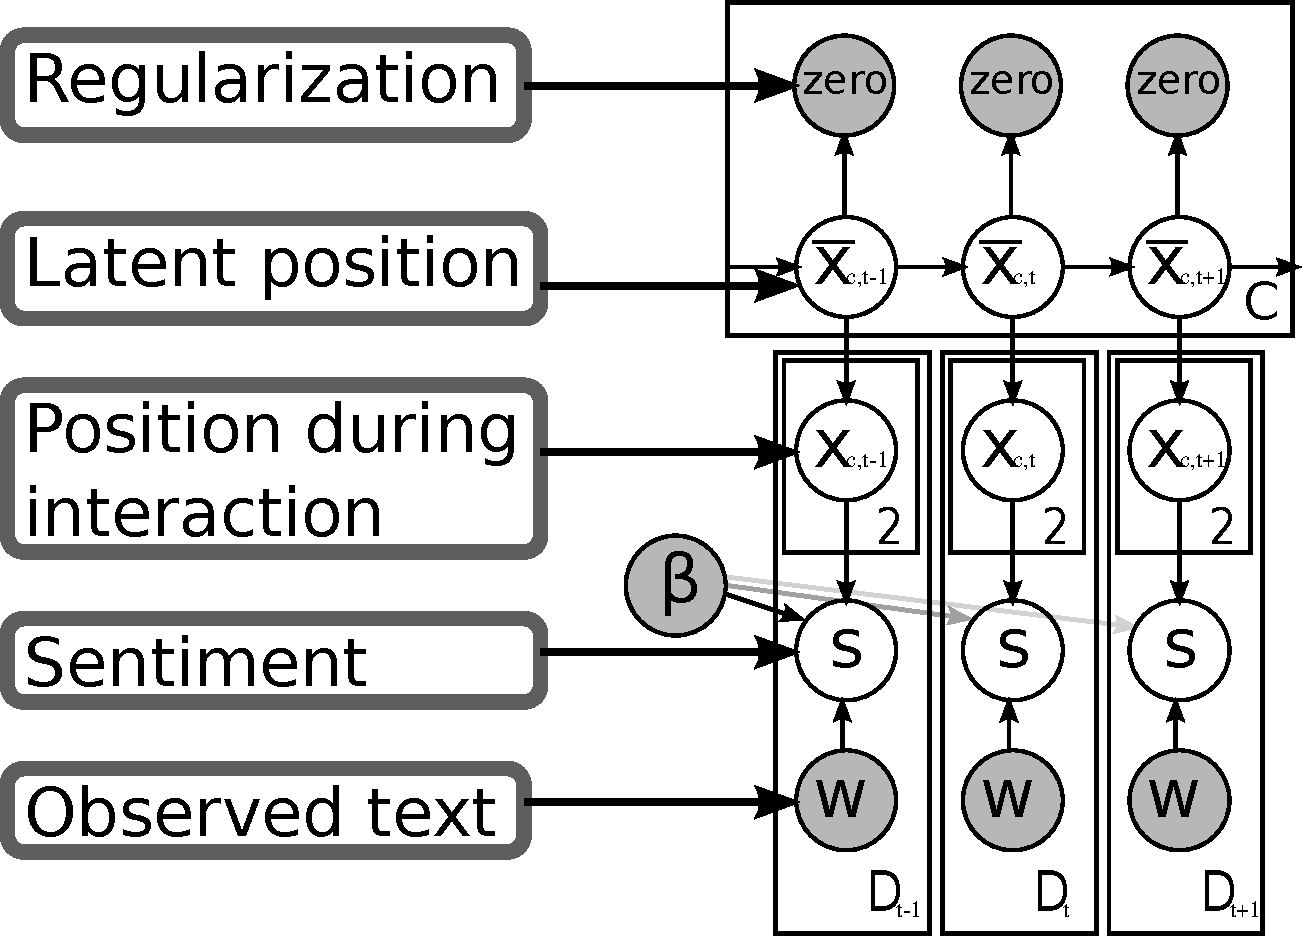
\includegraphics[width=0.3\textwidth]{chapter_foreign_relations/figures/countries_gm.pdf}
  \caption{A time-series model of countries' interactions.
    Pseudo-observations of ``zero'' are added for regularization.
    Amazon Mechanical Turk labels are used to fit $\beta$, which is
    used to infer unobserved sentiments.}
  \label{figure:gm}
  \vspace{-30pt}
\end{figure}
Reflecting the intuitions above, we assume that each nation lies in a
space of latent `''foreign sentiment''.  A spatial a model has two
benefits. First, it provides interpretability: nations with similar
positions in this latent space tend to interact more positively, while
nations further apart tend to have more tension in their relationship.
A spatial model also allows us to draw on ideas from
multidimensional scaling, which has been used successfully in both
political science \cite{martin:2002,jackman:2001} and social network
modeling \cite{hoff:2002,chang:2009}.

In the model we outline below, we assume that each country $c$ takes a
position $\bar x_c \in \mathcal{R}^P$ in the space of latent political
sentiment. The relationship between two countries will be determined
by the interaction of their positions $\bar x_c$.

\subsection{Related work}
% Covariates of war
% united nations general assembly

\paragraph{A temporal model of interaction.}
Foreign relations are not static, however; nations' alliances and
preferences change over time with the evolution of economies,
technology, and culture.  We make a further assumption that each piece
of news $d$ about two nations $c_1$ and $c_2$ reflects some underlying
sentiment $s_d$ between them.  We make this a fully temporal model by
allowing each country's mean position $\bar x_{c,t}$ to drift over
time with the Markov transition
\begin{align}
  \bar x_{ct} | \bar x_{c,t-1} \sim N(\bar x_{c,t-1}, \sigma_K^2),
\end{align}
as shown in Figure~\ref{figure:gm}. At any time $t$, state $c_1$ may interact with state $c_2$ in the following way:
\begin{align}
  x_{c_1,d} \sim N(\bar x_{c_1, t}, \sigma_D^2) \nonumber \\
  x_{c_2,d} \sim N(\bar x_{c_2, t}, \sigma_D^2) \nonumber \\
  s_d := x_{c_1,d}^T x_{c_2,d}, \nonumber \\
\label{equation:sentiment}
\end{align}
where we interpret $s_d$ as the sentiment between $c_1$ and $c_2$ as
reflected by article $d$.  When $c_1$ and $c_2$ are similar (as
measured by their inner product), their sentiment $s_d$ will be
positive; if they are dissimilar, their sentiment will be negative.
More extreme values indicate stronger sentiment.


\label{section:text_regression}
When a news source discusses the relationship between these nations,
the author's choice of words $\bm w_d$ reflects the relationship
between the countries.  We model this sentiment with the text of the
article $d$.  Using text regression \cite{kogan:2009}, the sentiment is modeled on wordcounts $\bm w_d$ of the article:
\[
  s_d | \bm w_d, \beta \sim \mathcal{N}( \bm w_d^T \beta , \sigma_W^2 ).
\]
We describe how to fit $\beta$ with Amazon Mechanical Turk workers in
Section~\ref{section:mturk}.

% In addition, a UN resolution may come up for vote at any time.  States
% cast a vote based on their current positions:
% \begin{align}
% x_{c_1,d} \sim N(\bar x_{c_1, t}, \sigma_D^2) \nonumber \\
% p(v_{cr}) = \sigma(x_{c_2, t} b_r + a_r) \nonumber \\
% \end{align}

% \begin{wrapfigure}{r}{0.4\textwidth}
%   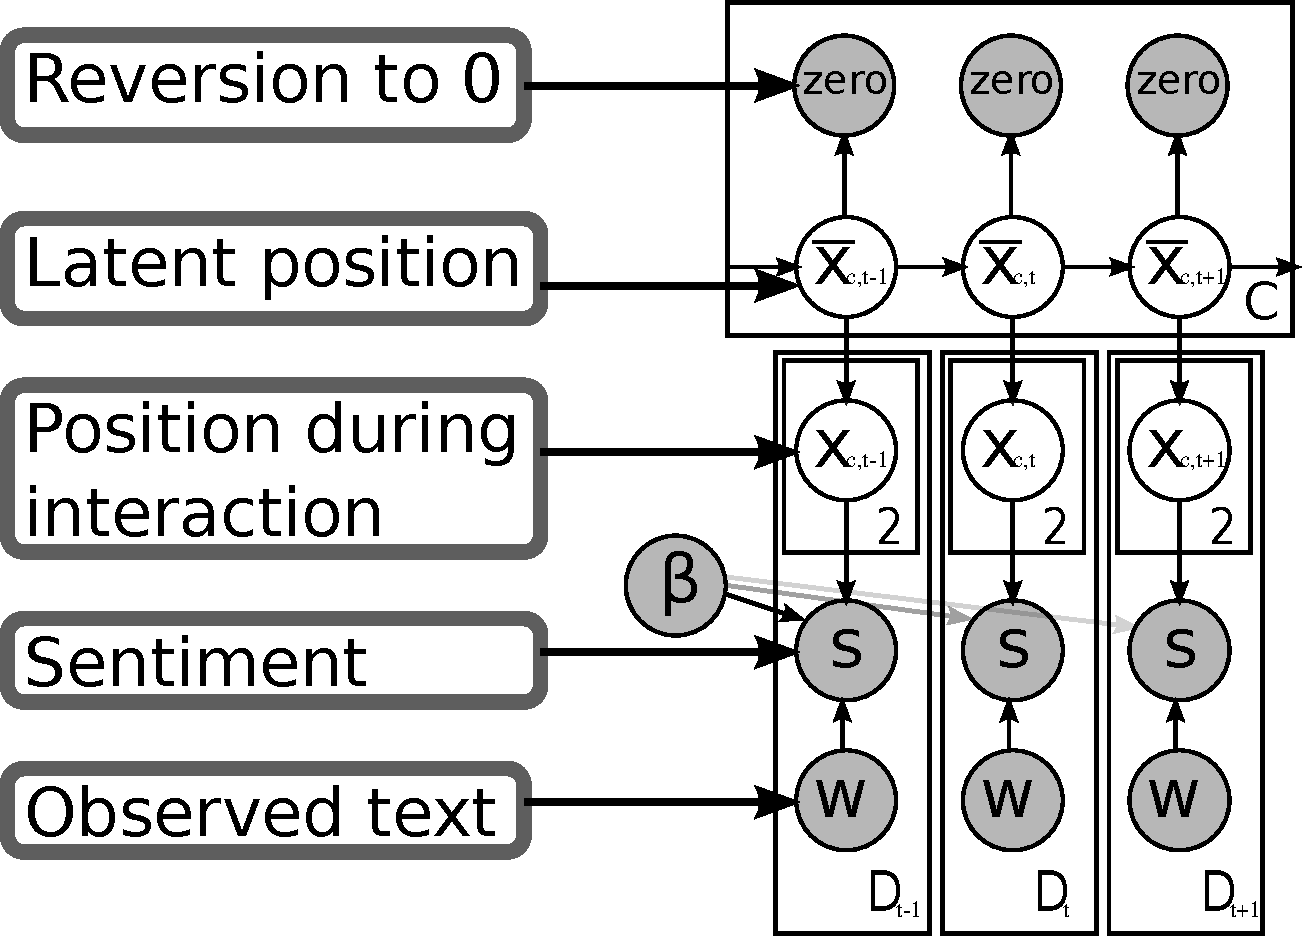
\includegraphics[width=0.4\textwidth]{figs/countries_gm.pdf}
%   \caption{The full time-series model of interaction by countries.
%     The large plate shows replication of a Markov chain for each
%     country.  Certain countries interact at each epoch -- possibly
%     multiple times -- with sentiment $s$.}
%   \label{fig:countries_by_ip}
% \end{wrapfigure}

\subsection{Related work}

% Democracy, Political Similarity, and International Alliances, 1816-1992
% Brian Lai
% Dan Reiterb
% Department of Political Science, Emory University
Spatial models such as Item Response Theory (IRT) have been developed
over the past century by quantitative social scientists for analyzing
behavior.  While much of this work has been used to model
parliamentary voting behavior, these techniques have also been used to
model voting in the UN General Assembly. Gartzke et al., for example,
use these votes and alliance models to study the nations' affinities
\cite{gartzke:1998}.

These models have been developed for dyadic data more fully in network
models such as the latent space model \cite{hoff:2002,sarkar:2005}, in
which the probability of a link between two nodes is a function of
their latent-space distance.  The qualitative relationship of
entities' dyadic relationships has been more fully developed with text
by the relational topic model, which uses free text to model the
relationship between actors in an unsupervised setting
\cite{chang:2009}.
% Supervised topic models


% Affinity of states dataset: 
% Fading Friendships (working paper)
% Alliances, Affinities and the Activation of International Identities∗
% Erik Gartzke†
% Alex Weisiger‡
% 7 March 2011

\section{Inference}
We fit the \emph{MAP} objective of this probabilistic model.  This has
the benefit of both clean exposition and simple implementation, and it
can be interpreted as a form of unregularized variational inference.
We optimize the \emph{MAP} objective in this model using traditional
EM.

\paragraph{M Step.} In the M step, the mean of each country's position
is updated using a modified Kalman filter.  This step differs from a
standard Kalman filter in that we may have no or multiple observations
on any given date.  We also add \emph{pseudo-observations} for each
country at each day $t$ with mean 0 and variance 10.  These
observations are a form of ``time-series regularization'' and reflect
the sense that a lack of news is effectively neutral news. The prior
over the ends of the chain are standard normal.

\paragraph{E Step.} In the E-step, our goal is to infer nations'
positions $x_{c,d} | \bar{x}_{c,t_d}, s_d$ with each interaction $d$ given
their means and the sentiment $s_d$ for this interaction.  We find
these positions by gradient ascent on $x_{c,d}$.

\section{Estimation of sentiment $s$}
\label{section:sentiment_models}
To infer the sentiment $s_d$ between two countries, we treat the
corresponding news article as a bag-of-words and use text regression
\cite{kogan:2009}.  In each of these cases, the sentiment $s_d$ is
first estimated on a training set using Amazon Mechanical Turk (AMT).
AMT is a crowdsourcing platform which provides access to thousands of
``workers'' who perform simple tasks over the Internet.  These labels
are then attached to all articles by predicting their sentiment.
